\documentclass[twocolumn]{article}
\usepackage[utf8]{inputenc}
\usepackage{enumerate}
\usepackage{amsmath}
\usepackage{graphicx}
\usepackage{listings}
\linespread{1.05}
\usepackage[sc]{mathpazo}
\usepackage{color}
\usepackage{gensymb}
\usepackage{multicol}
\usepackage{ltxgrid}
\usepackage{float}
\usepackage{romannum}
\usepackage{times}

\begin{document}
\title{\vspace{-2.5cm}FYS-3150 Prosjekt 1}
\author{Tobias Olesen & Thomas Sjåstad}
\date{13. September 2017}
\maketitle
\onecolumngrid
\noindent\makebox[\linewidth]{\rule{\paperwidth}{0.4pt}}
\begin{center}
\section*{SAMMENDRAG}
Løsningen av Poisson ligningen i én dimensjon numerisk viste seg å være god ved bruk av opptil $10^5$ gridpoints sammenlignet med analytisk løsning. Den numeriske presisjonen ble mistet etter dette ved valg av høyere n. Det ble funnet en minste relativ feil på størrelsesorden $10^{-8}$ med $10^5$ gridpoints. Metodene LU dekomposisjonon og tridiagonal matrise viste seg å ha stor differanse i CPU tid da LU dekomposisjons metoden tok en faktor $10^2$ ganger lenger tid enn tridiagonals metoden noe som skyldes antall flops for samtlige metoder.        
\end{center}  
\noindent\makebox[\linewidth]{\rule{\paperwidth}{0.4pt}}
\newline
\twocolumngrid
\section*{\Romannum{1}. INTRODUKSJON}
Det er flere formål med dette prosjektet, det ene er å få et overblikk over numerisk presisjon og hvor denne grensen er. Numerisk presisjon, forteller oss hvor godt vi er istand til å representere en løsning med en datamaskin. En datamaskin har en viss kapasitet til å representere tall til en viss presisjon (antall desimaler). Løsningen gjort på datamaskin skal sammenlignes med en analytisk løsning; To, beregne den relative feilen når antall trinn økes (steglengden minkes for å få en mer presis løsning relativt til den analytiske); Tre, løse en andre ordens differensial ligning ved bruk av LU dekomposisjon og ved radreduksjon av en tridiagonal matrise og se hvor lang tid PC'en bruker på disse metodene. Differensial ligningen som skal løses er den én-dimensjonale Poisson ligningen med Dirichlet grensebetingelser. Vi skal bruke metodene forover og bakover substitusjon for å løse Poisson ligningen numerisk. Forover og bakover substitusjon baserer seg på radreduksjon (Gauss eliminasjon) der forover sub eliminerer de første n-1 elementene i en nxn matrise og ser om det er en løsning. Bakover substitusjon finner løsningen dersom denne finnnes. LU dekomposisjon finner løsningen ved å dele opp matrisen i en nedre og en øvre triangulær matrise og ta determinanten. 
Med disse to metodene vil vi sammenligne tiden og nøyaktigheten. Tiden det tar for en datamaskin å fullføre en utregning av en ligning avhenger av hvor man FLOPS (floating point operations) som innholdes i uttrykket en vil løse. Eksempler på flops er deling, ganging, addering og subtraksjon.    
\section*{\Romannum{2}. METODE/FREMGANGSMÅTE}
Differensialligningen vi vil løse ser slik ut:
\begin{equation}
-u''(x) = f(x)
\end{equation}
Differensialligningen vår (Poisson-ligningen) kan omgjøres til et lineært ligningsett, som deretter kan løses ved Gauss-eliminasjon.
Først diskretiserer vi (1). Den andrederiverte av u kan da tilnærmes som:
\begin{equation}
-\frac{v_{i+1} + v_{i-1} - 2v_i} {h^2} = f_i
\end{equation}
hvor $i = 1, ..., n$, $f_i = f(x_i)$ og vi har definert steglengden $h = \frac{1}{n+1}$ (fra oppgaveteksten).
Ligning (2) kan da skrives som matriseligningen
\begin{equation}
\bold{A}\vec{v} = \vec{b}
\end{equation}
hvor $b_i = h^2 f_i$.
\subsection*{Gauss eliminasjon}
Ligning (3) gir oss følgende system (gitt et 4x4-tilfelle):
$$a_{11}v_1 + a_{12}v_2 + a_{13}v_3 + a_{14}v_4 =b_1$$
$$a_{21}v_1 + a_{22}v_2 + a_{23}v_3 + a_{24}v_4 =b_2$$
$$a_{31}v_1 + a_{32}v_2 + a_{33}v_3 + a_{34}v_4 =b_3$$
$$a_{41}v_1 + a_{42}v_2 + a_{43}v_3 + a_{44}v_4 =b_4$$

Den generelle ideen bak Gauss eliminasjon er så å bruke den første ligningen til å eliminere den første ukjente $v_1$ fra de siste n-1 ligningene, for så å bruke den nye (andre) ligningen til å eliminere den andre ukjente $v_2$ fra de gjenværende n-2 ligningene. Med n-1 slike eliminasjoner vil man sitte igjen med et såkalt øvre triangulært ligningssett (bare nuller under hoveddiagonalen). Dette kalles også en framover-substitusjon. Det andre trinnet i metoden er en bakoversubstitusjon som vil gi oss løsningen.

\subsection*{Generell framover-substitusjon}
Algoritmen vår for framover-substitusjon (for et generelt system) er altså basert på Gauss eliminasjon, og blir implementert i koden vår med en for loop over elementene $i$. For hver i oppdateres så diagonalelementene $b_i$ med de nye diagonalelementene $\tilde{b_i}$:

\begin{equation}
\tilde{b_i} = b_i - \frac{a_i c_{i-1}}{\tilde{b_{i-1}}}
\end{equation}

Den nye høyresiden $\tilde{f_i}$ er da gitt ved:

\begin{equation}
\tilde{f_i} = f_i - \frac{a_i \tilde{f_{i-1}}}{\tilde{b_{i-1}}}
\end{equation}

\subsection*{Generell bakover-substitusjon}
Bakover-substitusjonen gir oss så den endelige løsningen:

\begin{equation}
u_{i-1} = \frac{\tilde{f_{i-1}} - c_{i-1} u_i}{\tilde{b_{i-1}}}
\end{equation}

hvor $u_n = \tilde{f_n}/ \tilde{b_n}$ når $i = n$.

\begin{figure}[h!]

  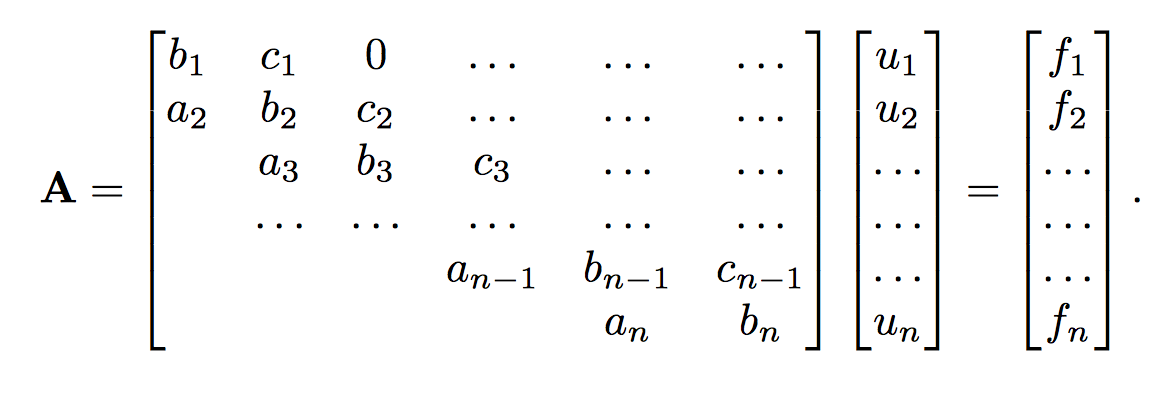
\includegraphics[width=\linewidth]{pict_1.png}
  \caption{Ligningssystemet med generell tridiagonal matrise A}
\end{figure}

\subsection*{Spesiell framover-substitusjon}
For vår spesifikke andrederiverte av u så får vi også en spesifikk tridiagonal matrise A. Denne matrisen har identiske elementer langs hele hoveddiagonalen samt identiske (men forskjellige) elementer både på diagonalen rett ovenfor og rett nedenfor hoveddiagonalen. Dette faktum kan brukes til å lage en algoritme spesifikt for A, som også består av en framover- og bakover-substitusjon henholdsvis. Framover-substitusjonen gir oss matrisens nye diagonalelementer $\tilde{d_i}$:


\begin{equation}
\tilde{d_i} = 2 - \frac{1}{\tilde{d_{i-1}}} = \frac{i+1}{i}
\end{equation}
samt den nye høyresiden $\tilde{f_i}$ av ligningen:
\begin{equation}
\tilde{f_i} = f_i + \frac{(i-1)\tilde{f_{i-1}}}{i}
\end{equation}

\begin{figure}[h!]
  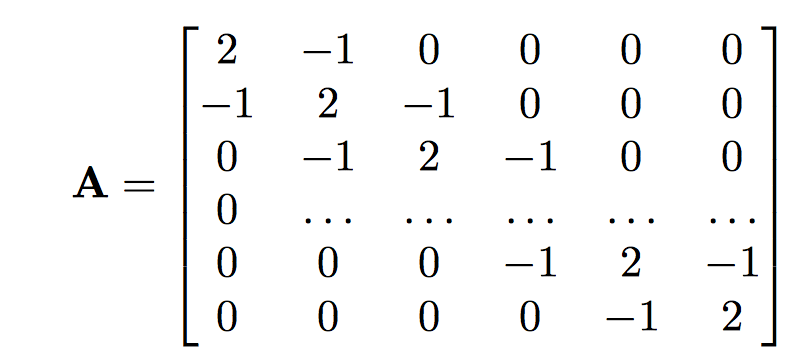
\includegraphics[width=\linewidth]{pict_2.png}
  \caption{Den spesielle tridiagonale matrisen}
\end{figure}

\subsection*{Spesiell bakover-substitusjon}
Bakover-substitusjonen gir oss nok en gang den endelige løsningen:

\begin{equation}
u_{i-1} = \frac{i-1}{i} (\tilde{f_{i-1}} + u_i)
\end{equation}

med $u_n = \tilde{f_n} / \tilde{b_n}$.

\subsection*{Relativ feil}
Vi er også interesserte i å kalkulere den relative feilen i resultatene for å kunne sammenligne den numeriske løsningen vår $v$ med den analytiske løsningen $u(x)$.
Den relative feilen er gitt ved:
\begin{equation}
\epsilon_i=log_{10}\left(\left|\frac{v_i-u_i}
                 {u_i}\right|\right)
\end{equation}

hvor $u(x) = 1-(1-e^{-10})x-e^{-10x}$.
\newpage
\section*{\Romannum{3}. RESULTATER}
\textbf{Link til programmer:}
\newline
https://github.com/tobiasolesen/FYS3150-Prosjekt-1
\begin{figure}[H]
\centering
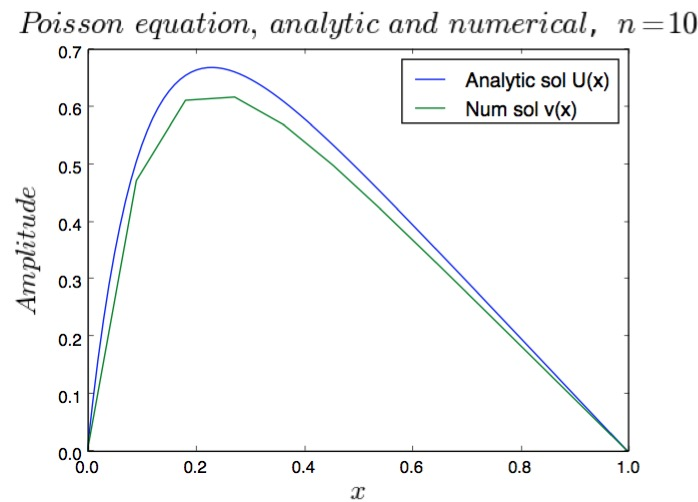
\includegraphics[width=8cm]{1a_n_10.jpg}
\caption{Løsningen v(x) med 10 datapunkter av ligningen $Av = B$ (hvor v er løsningen) som er plottet med den analytiske U(x) med grensebetingelser.}
\end{figure}
\begin{figure}[H]
\centering
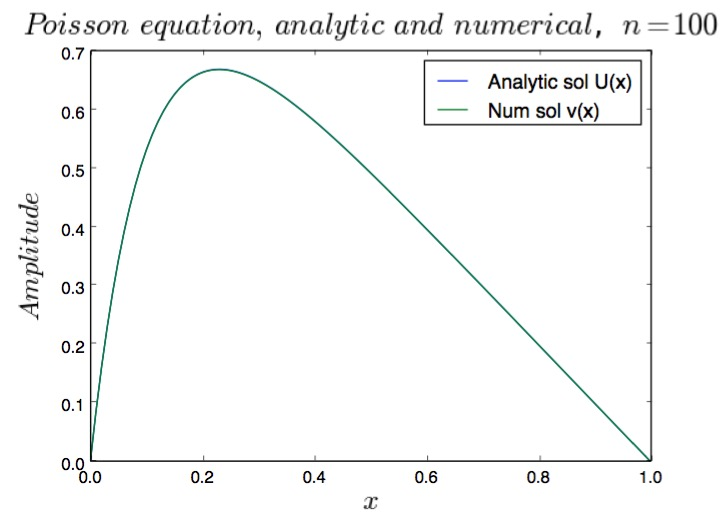
\includegraphics[width=8cm]{1a_n_100.jpg}
\caption{Samme som i figur 1, men med 100 datapunkter. Analytisk og numerisk løsning ligger nærme hverandre}
\end{figure}
\begin{figure}[H]
\centering
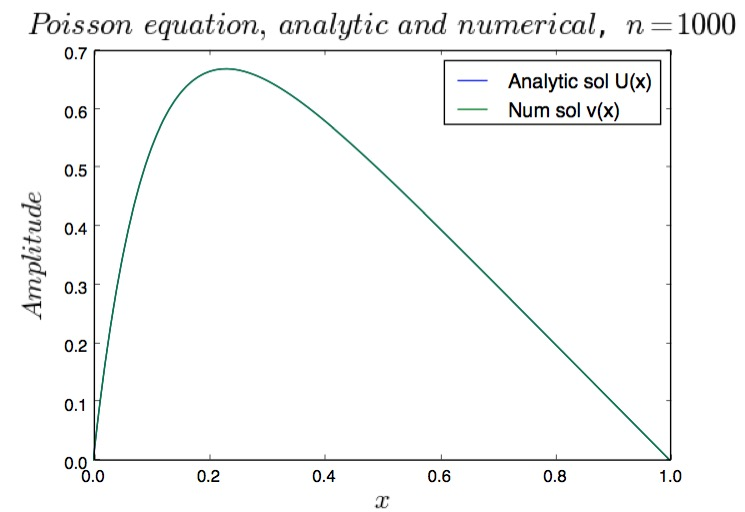
\includegraphics[width=8cm]{1a_n_1000.jpg}
\caption{Tilslutt vises ett plot med 1000 datapunkter hvor vi ser at den numeriske og analytiske ligger så å si oppå hverandre.}
\end{figure}
\subsection*{FLOPS}
Antall flops som trengs for algoritmene i programmet, forover- og bakover substitusjonen fant vi til å være 4(n-1) for forover sub og 2(n-1) for bakover. n er her antall gridpoints (datapunkter). 
\subsection*{CPU tid}
\textbf{Tabell 1: Sammenligning av CPU tid for det generelle og spesielle tifelle fant vi at:} 
\bigskip
\resizebox{8cm}{!} {
\begin{tabular*}{0.6\textwidth}{@{\extracolsep{\fill} } | c | c | c |  }
  \hline
  \textbf{Antall n}  & \textbf{Generell tid [s]}  & \textbf{Spesiell tid [s]}\\
  \hline 
  10 & 2e-4 & 2e-4 \\
  \hline
  100  & 1e-3  & 1.4e-3 \\
  \hline
  1e3  & 1.4e-2 & 1.7e-2 \\
  \hline
  1e4  & 0.13 & 0.14\\
  \hline
  1e5  & 1.53 & 1.47\\
  \hline
  1e6  & 17.7 & 17.7\\
  \hline
\end{tabular*}
}
\newpage

\subsection*{Relativ feil}
\textbf{Tabell 2: Tabell som viser størrelsesorden av den relative feilen for forskjellige valg av n:}
\bigskip
\resizebox{8cm}{!} {
\begin{tabular*}{0.6\textwidth}{@{\extracolsep{\fill} } | c | c |  }
    \hline
    \textbf{Antall n} & \textbf{Relativ feil} \\
    \hline 
    10 & -1   \\
    \hline
    100  & -3 \\
    \hline
    1e3  & -5 \\
    \hline
    1e4  & -7 \\
    \hline
    1e5  & -8 \\
    \hline
    1e6  &  -6\\
    \hline
\end{tabular*}
}
\bigskip
Prøvde å øke n til 1e7, men fikk memoryerror. Fikk ikke tatt med denne feilen.
\subsubsection*{Tabell 3: LU og tridiagonal tid:}

\bigskip
\resizebox{8cm}{!} {
\begin{tabular*}{0.6\textwidth}{@{\extracolsep{\fill} } | c | c | c |  }
  \hline
  \textbf{Antall n}  & \textbf{LU tid [s]}  & \textbf{Tridiagonal tid [s]}\\
  \hline 
  10 & 5e-4 & 2e-4 \\
  \hline
  100  & 4e-3  & 1.4e-3 \\
  \hline
  1e3  & 0.3 & 1.7e-2 \\
  \hline
  1e4  & 88 & 0.14 \\
  \hline
\end{tabular*}
}
\subsubsection*{Tabell 4: Sammenligning av LU og Tridiagonal resultat.}

\bigskip
\resizebox{8cm}{!} {
\begin{tabular*}{0.6\textwidth}{@{\extracolsep{\fill} } | c | c |  }
  \hline
  \textbf{Antall n}  & \textbf{Differanse} \\
  \hline 
  10 & 1.2 \\
  \hline
  100  & 0.09 \\
  \hline
  1e3  & 0.009 \\
  \hline
  1e4 & 0.0009 \\
  \hline
\end{tabular*}
}
\section*{\Romannum{4}. DISKUSJON} 
Fra figur 2 og 3 ser vi at den numeriske løsningen er en veldig god tilnærming til den analytiske. Det er liten forskjell i løsningen fra 100 - 1000 gridpoints. 

Antall flops som var nødvendig ble redusert med to for begge substutisjonene da det var av fordel å beregne diagonalelementene (2'ere og -1'ere) i en egen løkke. Dette sparte oss noe CPU tid. Tiden for den generelle matrisen og spesielle matrisen samsvarer noe som ikke er helt forventet da den spesielle matrisen trengte færre beregninger fordi matrisen innholdt mange nullere imotsetning til den generelle matrisen. Denne sammensvarelsen kan skyldes andre programmer som kjører ved siden av  . Den tiden det har tatt har muligens vært påvirket av andre programmer slik at tiden har vist samme tid. 

Den numeriske presisjon svikter for n = 1e6 fra tabell 2 da vi har en trend fra n = 10 til n = 1e5 hvor den relative feilen blir mindre, men etter det blir den større. Datamaskinen er ikke istand til å representere tallene produsert med denne "oppløsning" og tallene blir rundet av. Med denne presisjonsen vil avrundingen sørge for at feilen blir større.

LU dekomposisjonen ser vi fra tabell 3 tar lengre tid å kalkulere enn tridiagonal tiden etterhvert som n øker. Fant at antall flops for tridiagonal matrisen var $2(n-1)$ og $4(n-1)$, men s antall flops for LU dekomposisjonen er på en størrelsesorden av $n^3$. Dette forklarer den store økningen i beregningstid. Når n øker med en faktor 10 så burde det forventes tiden det vil ta økes med faktor på $10^3$. Fra tabell 3 ser dette ikke helt ut til å stemme da det er en endring med en størrelsesorden $10^2$. Metodene ser ut til å nærme seg samme resultat for økning av n fra tabell 4.     
\section*{\Romannum{5}. KONKLUSJON}
Løsningene numerisk og analytisk stemte godt overens og tiden det tok for å få relativt godt resultat var liten. 
Antall flops har stor påvirkning på tiden til algoritmene som har blitt kjørt og i noen tilfeller kan antall flops reduseres, her ble antall flops redusert fra 6 til 4 og fra 4 til 2.
Den relative feilen hadde en god numerisk presisjon ved valg av $n = 1e5$, etter dette ble det tap på numerisk presisjon. Tilslutt viste LU dekomposisjonens algoritmen å ta betydelig lenger tid enn tridiagonal matrisen hvor forskjellen på størrelsesorden var på $10^2$ for n = 1000 og n = 10000, derimot resultatene viste seg å synke med en faktor 10 for hver økning av n med en faktor 10. 
\newpage

\section*{\Romannum{6}. REFERANSER}
Hjort -Jensen Morten., 2015. Computational Physics Kompendiet. 
\newline
http://compphysics.github.io/ComputationalPhysics/doc/pub/linalg/pdf/linalg-print.pdf 
\end{document}